\chapter{ELMy H-Modes on C-Mod}\label{ch:Elmy}

The ELMy H-mode \cite{Wagner1982,Keilhacker1984}, described in \cref{sec:hcr_elmy}, is the most commonly-accessed high-performance regime on major tokamak experiments.  The bursty transport driven by ELMs provides sufficient relaxation of the particle confinement in H-mode to allow stationary operation without excessive impurity accumulation; as such, the ELMy H-mode is considered the baseline operating regime for ITER \cite{ITER1999,Shimada2007}.  However, on ITER-scale devices the pulsed heat loading associated with ELMs drives unacceptable levels of erosion and damage to plasma-facing wall and divertor materials \cite{Loarte2003,Federici2003}.

In light of the impact of large, deleterious ELMs on the ITER wall, and the profound impact of pedestal height on overall plasma performance \cite{Kinsey2011,Doyle2007}, a firm understanding of the physics governing the pedestal in high-performance regimes and their extrapolation to reactor-scale devices is of paramount importance to fusion research leading up to ITER operation.  To that end, a Joint Research Target combining theory, experiment, and modeling efforts in the ELMy H-mode pedestal was undertaken \cite{Groebner2013}\gnote{cite tech report too?}.  Notably, this effort saw the development of the EPED model \cite{Snyder2009,Snyder2011,Snyder2009a}, described in \cref{sec:mod_eped}, which predicts the pressure pedestal width and height preceding the ELM crash through a combination of constraints based on peeling-ballooning MHD instability \cite{Snyder2004,Wilson2002,Wilson2006} (\cref{sec:mod_pb}) and kinetic-ballooning turbulence \cite{Snyder2001} (\cref{sec:mod_turbulence}).  In this chapter, we detail the contributions from Alcator C-Mod to this joint effort \cite{Walk2012}\gnote{how to emphasize my own contribution?} both in empirical studies of the ELMy H-mode pedestal, and in the implementation of the EPED model.  C-Mod ELMy H-modes greatly expand the parameter space in which the EPED model is tested, reaching within a factor of two of the target pedestal pressure for ITER.  The techniques developed in this analysis will subsequently be applied to I-mode pedestals\gnote{reword}.\nicesectionending

\section{ELMy H-Mode Access \& Experimental Arrangement}\label{sec:elmy_access}

\begin{figure}[t]
 \pushtooutside
 \fcapside[55mm]{\caption{C-Mod cross-section comparing the typical plasma shape (blue) to the altered shape favoring ELMy H-mode operation (red), developed in joint experiments with the JFT-2M tokamak \cite{Hughes2013}.  ELMy H-mode access is favored by high lower triangularity and an outer strike point in the divertor slot, coupled with very low upper triangularity and elongation.  This is thought to reduce the required edge pressure gradient and current to reach the peeling-ballooning boundary.}\label{fig:elmy_shaping}}{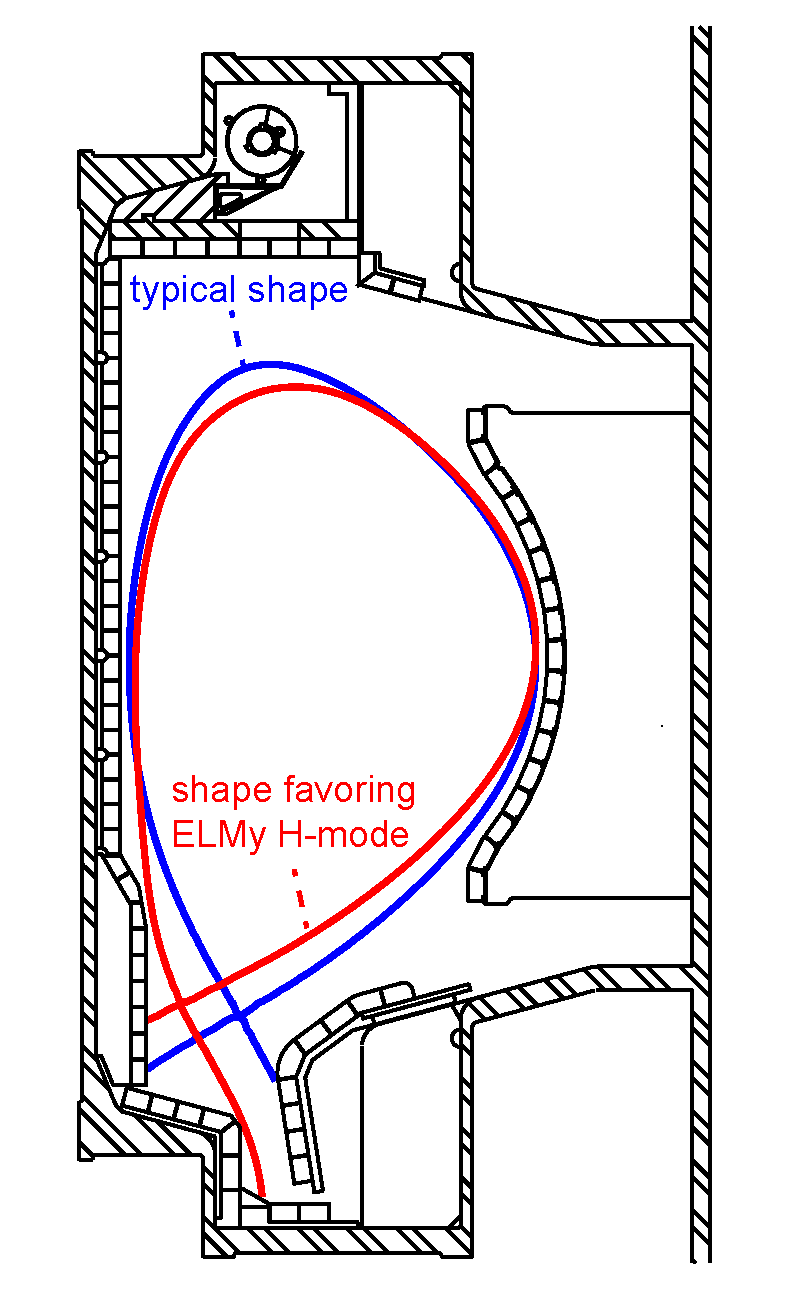
\includegraphics[width=90mm]{graphics/ELMy/shaping.pdf}}
\end{figure}

High-confinement operation on Alcator C-Mod differs is unique among major tokamak experiments in that typical H-modes do not exhibit the large Type-I ELMs\gnote{cite for this?} customarily seen on other devices.  Instead, ELM-free H-modes tend to form at lower collisionalities heating power levels, with high-density, high-power operation tending towards the continuously-regulated EDA H-mode rather than exhibiting discrete ELMs (see \cref{sec:hcr_elmfree,subsec:hcr_eda}).  However, by operating in a modified shape (see \cref{fig:elmy_shaping})\gnote{shape range} with low elongation and upper triangularity paired with high lower triangularity and a strike point on the divertor floor, regular ELMy H-mode operation is attainable.  This comparatively weak shaping, developed in similarity experiments with the JFT-2M tokamak \cite{Hughes2011}\gnote{better cite, Terry paper?}, reduces the necessary pressure gradient and bootstrap current to reach the ideal peeling-ballooning MHD stability boundary (described in \cref{sec:mod_pb}), triggering the ELM.  In this shape, new experiments on C-Mod \cite{Walk2012} attained ELMy H-modes across a broad range in current ($400-1100 \;\si{\kilo\ampere}$) and field ($3.5-8 \;\si{\tesla}$) with high-resolution pedestal data.

\begin{figure}[t]
 \pushtooutside
 \ffigbox[\FBwidth]{
\includegraphics[width=150mm]{graphics/ELMy/time_window.pdf}}{\caption{Example ELMy H-mode window (highlighted).  Phases for study are selected for steady density ($\overline{n}_e$ shown in the top trace), temperature (ECE $T_e$ signals shown for the core and pedestal), and ELM cycles ($D_\alpha$ signal shown).  The same modeling window is shown zoomed-in at the right.  Note the strong perturbation to the edge temperature due to the sawtooth crash.  Thomson scattering frames are indicated by the black ticks on the axes -- the ELM cycle is at a comparable frequency, $\sim \SI{60}{\hertz}$, to the TS system frame rate.  This presents a difficulty for selecting data masked to the ``peak'' of the ELM cycle, necessitating long, steady ELMing phases for study.}\label{fig:elmy_timewindow}}
\end{figure}

\begin{figure}
 \pushtooutside
 \ffigbox[\FBwidth]{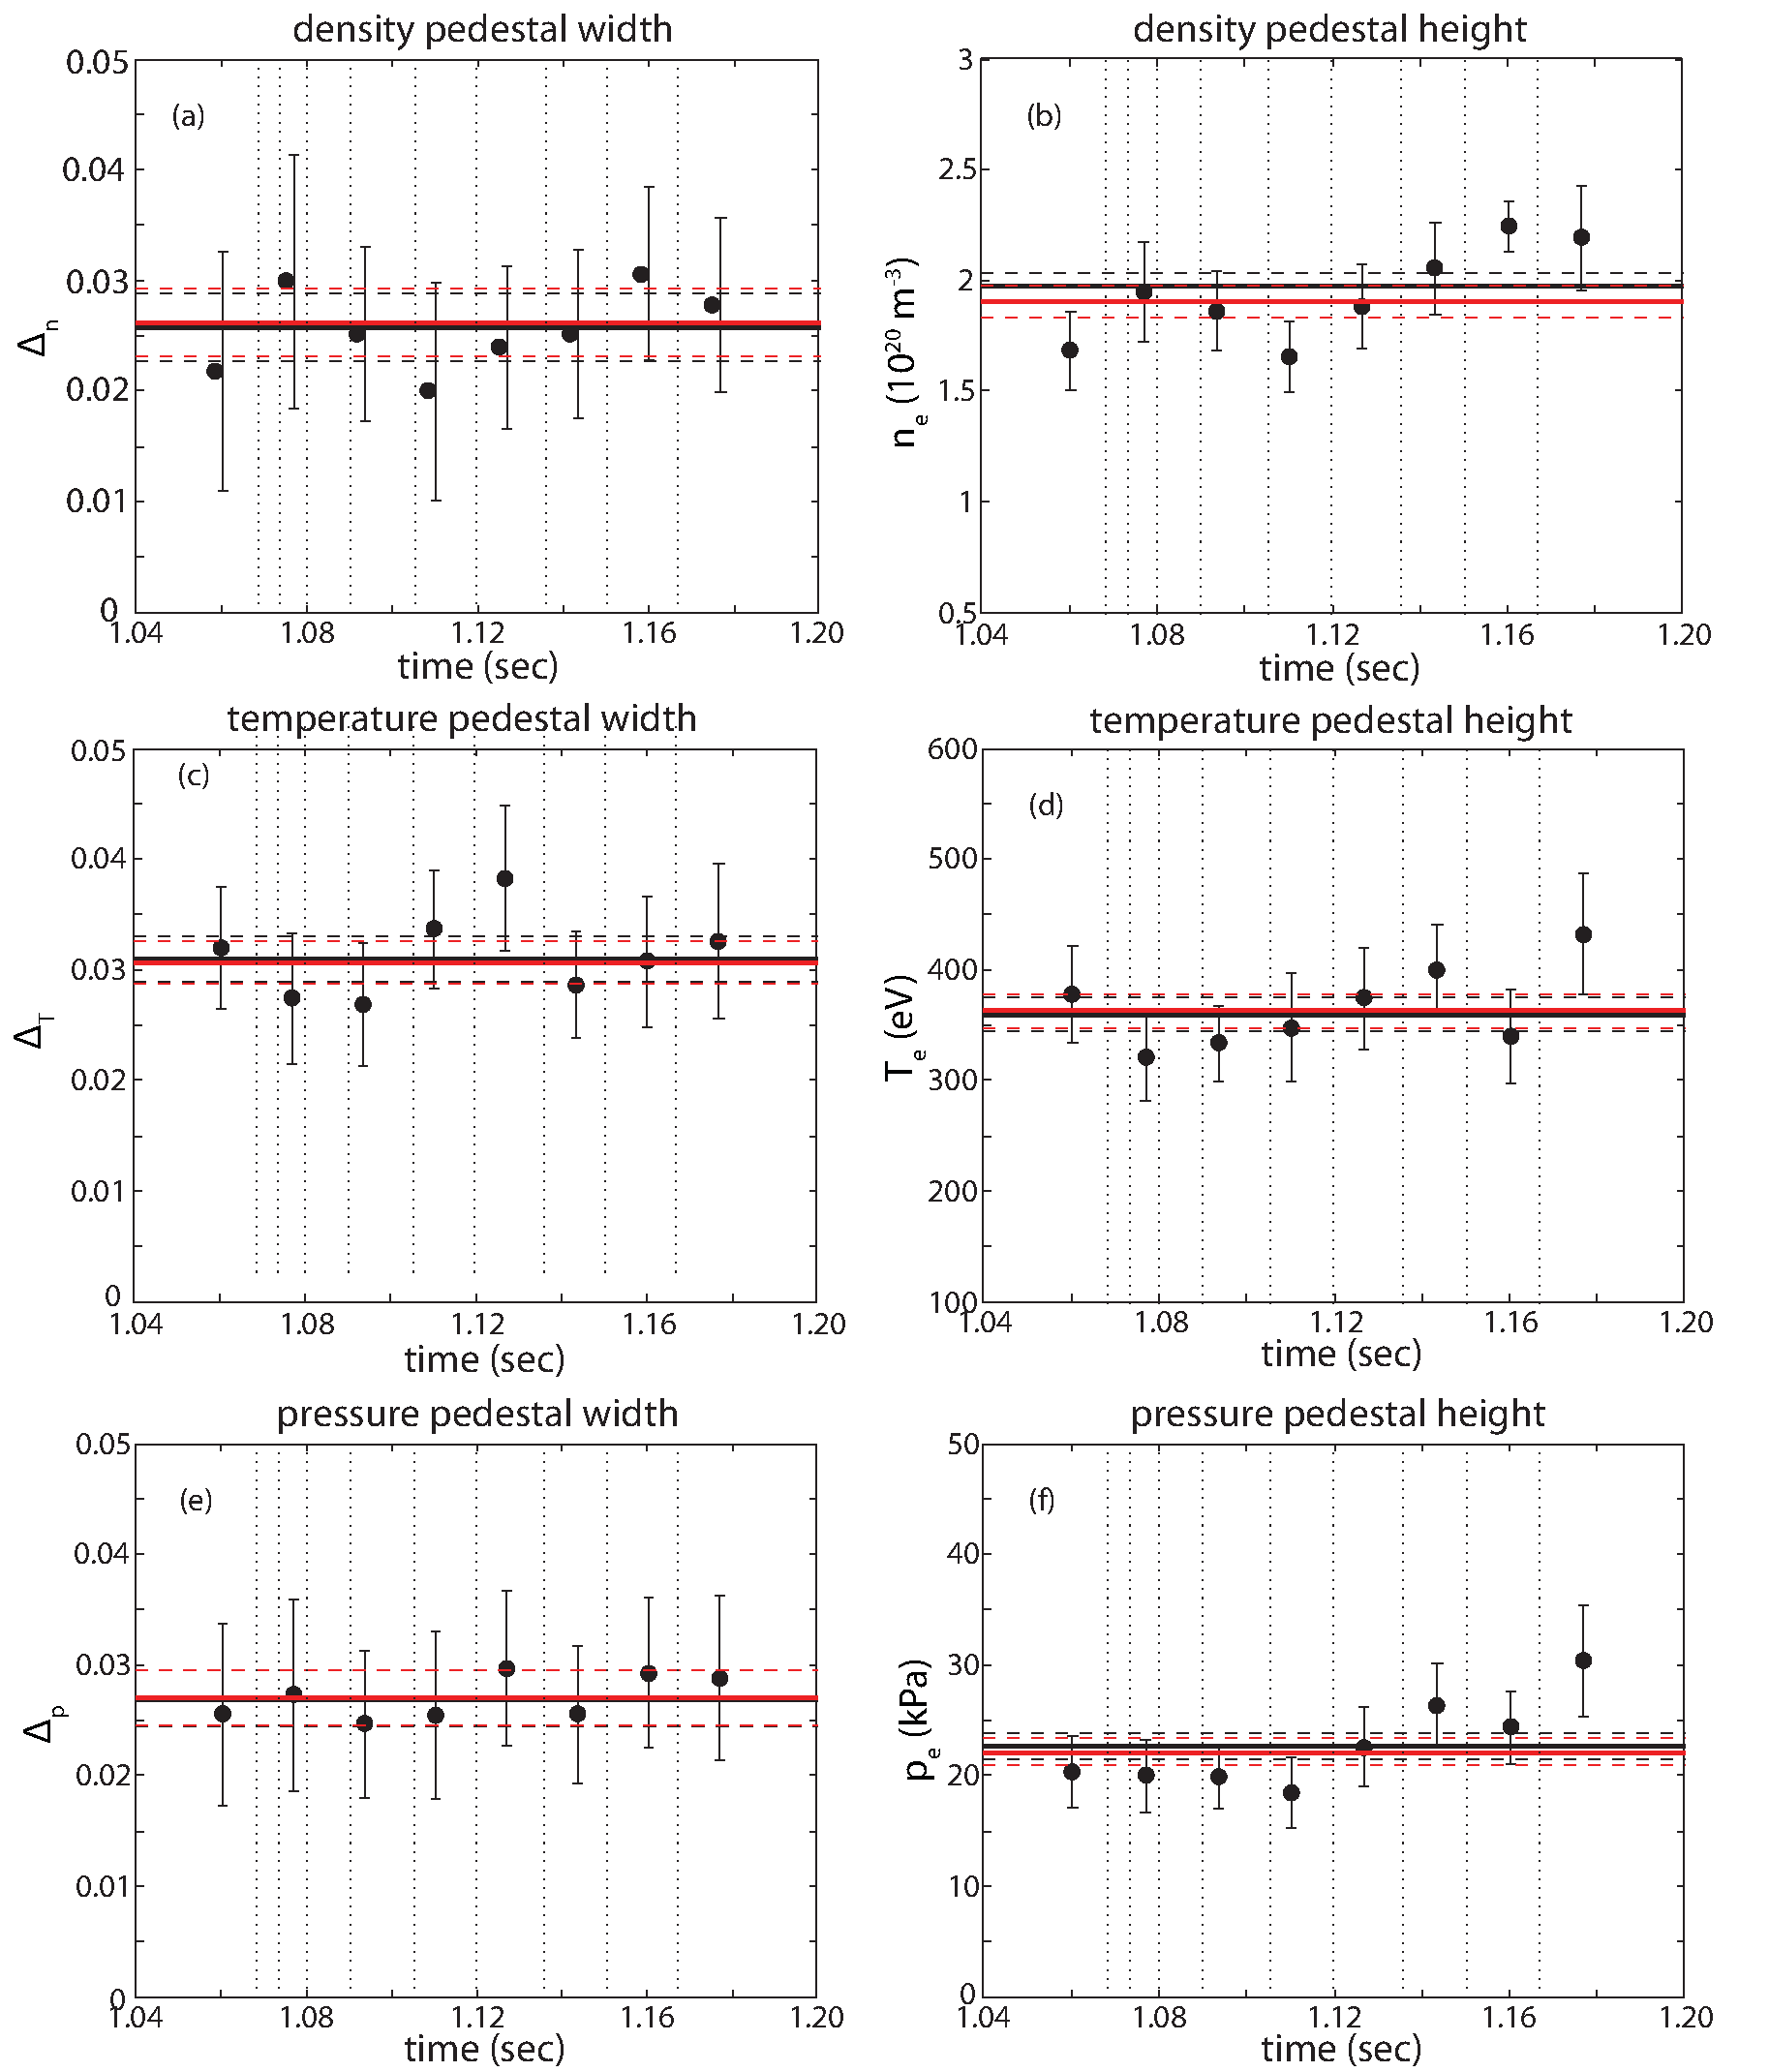
\includegraphics[width=150mm]{graphics/ELMy/ensemble.pdf}}{\caption{Comparison of fits for the $n_e$, $T_e$, and $p_e$ pedestal width and height from Thomson scattering.  Individual frames of data are shown as black points, with their average shown by the black line (errorbars indicated by the dashes).  The ensemble-averaged fit is shown in red.  The ensemble fit captures the average behavior in a steady ELMing phase well, while suppressing the random scatter found in indivual frames of TS data.  For comparison, ELM crash times in the window are indicated by vertical dashed lines.}\label{fig:elmy_ensemble}}
\end{figure}


Pedestal profiles are taken with the edge Thomson scattering system, detailed in \cref{subsec:app_ts_cmod}.  The pedestal data is taken over steady ELMing phases to minimize the effects of random scatter in the data -- an example of such a window, with line-averaged density $\overline{n}_e$, core and edge $T_e$, and divertor $D_\alpha$ signal (indicative of the ELM crash), is shown in \cref{fig:elmy_timewindow}, with a comparison of the individual-frame fits to the ensemble shown in \cref{fig:elmy_ensemble}.  Strictly, models of the pedestal structure in ELMy H-mode predict the pedestal immediately preceding the ELM crash, when the pedestal is most unstable to the ELM trigger.  However, ELMs on C-Mod typically cycle at $60-100 \;\si{\hertz}$, comparable to the repetition rate of the Thomson scattering system (as shown in \cref{fig:elmy_timewindow,fig:elmy_ensemble}).  This presents difficulties in resolving the pedestal with multiple frames per ELM and binning the data to the peaks of the ELM cycle.  In most cases, pedestals are prepared in a single ``ensemble average'' utilizing all TS data in the window; in certain cases, a statistical set is also constructed using the last 20\% of the ELM cycle as is typical for other machines.  The results from this correction are discussed in \cref{sec:elmy_sync}.

\begin{figure}
 \pushtooutside
 \fcapside[65mm]{\caption{Example pedestal illustrating the $mtanh$ function used for pedestal fitting (\cref{eq:mtanh}), defining the parameters: height $h$, baseline $b$, midpoint $x_0$, half-width $\delta$/full width $\Delta$.  The inboard slope is characterized by the parameter $\alpha$.}\label{fig:mtanh}}{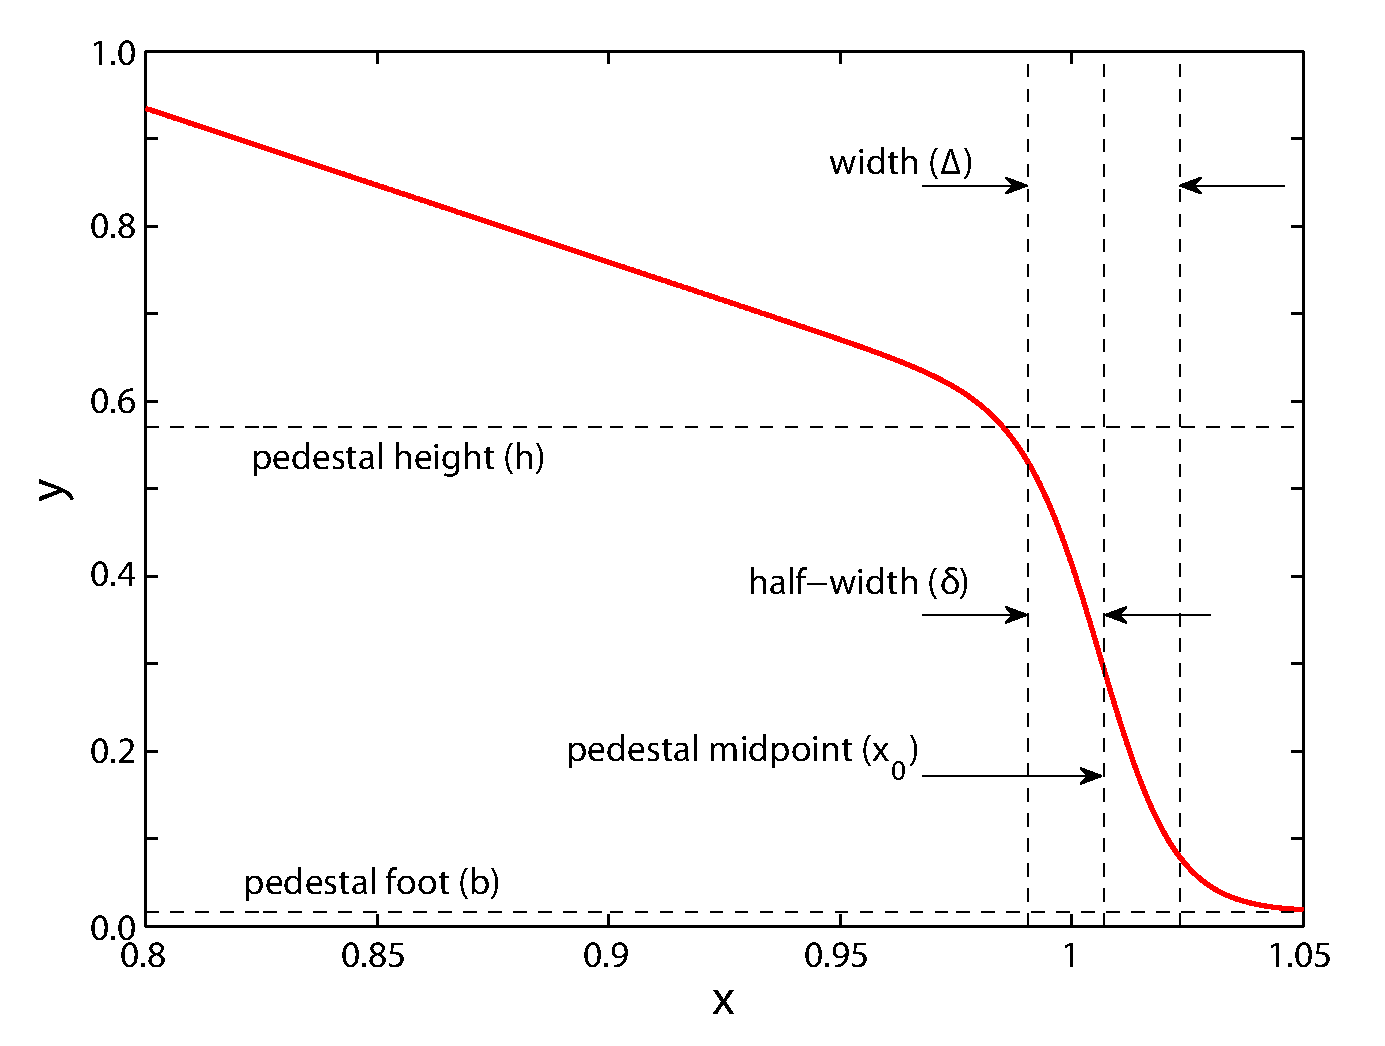
\includegraphics[width=100mm]{graphics/ELMy/mtanh.pdf}}
\end{figure}

The electron density, temperature, and pressure profiles are fitted using a modified hyperbolic-tangent fit developed in \cite{Groebner2001}.  In a general $x,y$ space, the fitting function is expressed by

\begin{equation}\label{eq:mtanh}
 \begin{aligned}
  z &= \frac{x_0 - x}{\delta}\\
  mtanh(\alpha,z) &= \frac{(1 + \alpha z) e^z - e^{-z}}{e^z + e^{-z}}\\
  y &= \frac{h+b}{2} + \frac{h-b}{2} mtanh(\alpha,z)
 \end{aligned}
\end{equation}

\noindent where $x_0$ is the pedestal midpoint, $h$ and $b$ are the height and baseline, and $\delta$ is the half-width (we use $\Delta = 2\delta$ as the ``pedestal width'').  The inboard slope is encoded by the parameter $\alpha$, with the multiplicative factor $1 + \alpha z$ providing an approximately linear profile inboard from the steep-gradient region.  This definition provides a smooth, continuous definition for the pedestal gradient throughout the profile, with the peak gradient found analytically at $x_0$.  Recent H-mode studies use the fitting parameter $h$ as the figure-of-merit for the pedestal height; however, it is also common to express the pedestal height in terms of the evaluated value of the fit at the 95\% poloidal flux surface.  For the purposes of this document we denote the height taken from the fitting parameter $h$ by the subscript $ped$, and values taken at the 95\% flux surface by the subscript $95$. 

Due to the ready availability of high-resolution electron density and temperature diagnostics, for the purposes of this section we assume equal ion and electron pressures, $p = 2n_e T_e$ (a viable approximation on C-Mod due to the relatively low impurity content found in ELMy H-modes, $Z_{eff} \sim 2$, and rapid ion-electron equilibration in H-mode pedestals on C-Mod\gnote{cites for this, elaborate}).  All profiles are prepared using normalized poloidal flux for the abscissa, facilitating comparison to results from other machines and to the EPED model.  For the purposes of the EPED model we also prepare an averaged width, defined by

\begin{equation}\label{eq:wid_eped}
  \delta_\psi = \frac{\delta_{n_e} + \delta_{T_e}}{2}\qquad
  \Delta_\psi = 2\delta_\psi
\end{equation}

\noindent a practice necessitated by the distinct measurements of $n_e$ and $T_e$ on certain machines\gnote{reword}.  As the density and temperature widths are quite close (although the density pedestal is, on average, slightly wider, as shown in \cref{fig:elmy_deltan_deltaT}\gnote{get value for this}), the difference between $\Delta_\psi$ and the directly-measured $\Delta_{p_e}$ is minimal -- as shown in \cref{fig:elmy_deltap_deltapsi}, the two widths are well-correlated, with $\Delta_\psi$ systematically somewhat wider.\nicesectionending

\begin{figure}
 \pushtooutside
 \begin{floatrow}
  \ffigbox[\FBwidth]{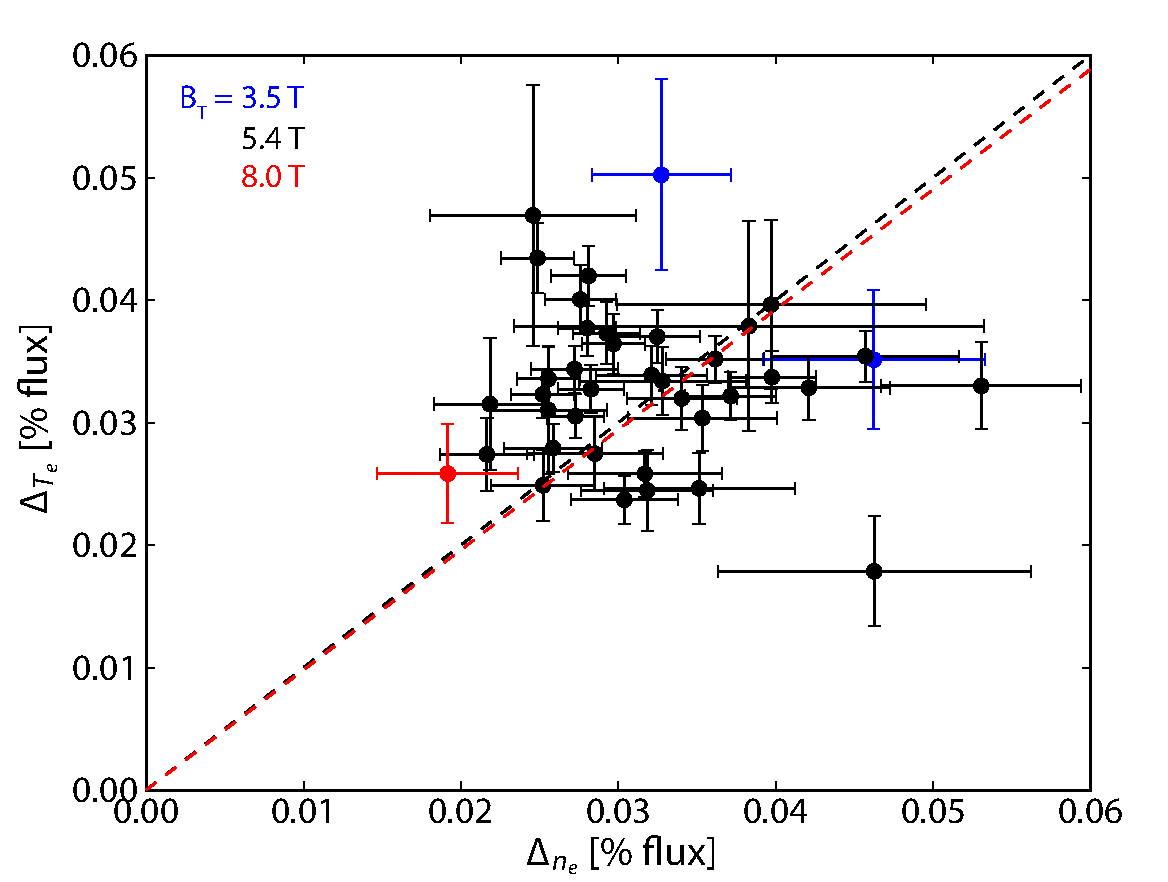
\includegraphics[width=75mm]{graphics/ELMy/deltan_deltaT.pdf}}{\caption{Comparison of the measured pedestal widths for the $n_e$ and $T_e$ pedestals, differentiated for the low-, standard-, and high-field H-mode cases.  Pedestal widths are similar for density and temperature, although on average the density pedestal is somewhat wider \note{measure!}}\label{fig:elmy_deltan_deltaT}}
  \ffigbox[\FBwidth]{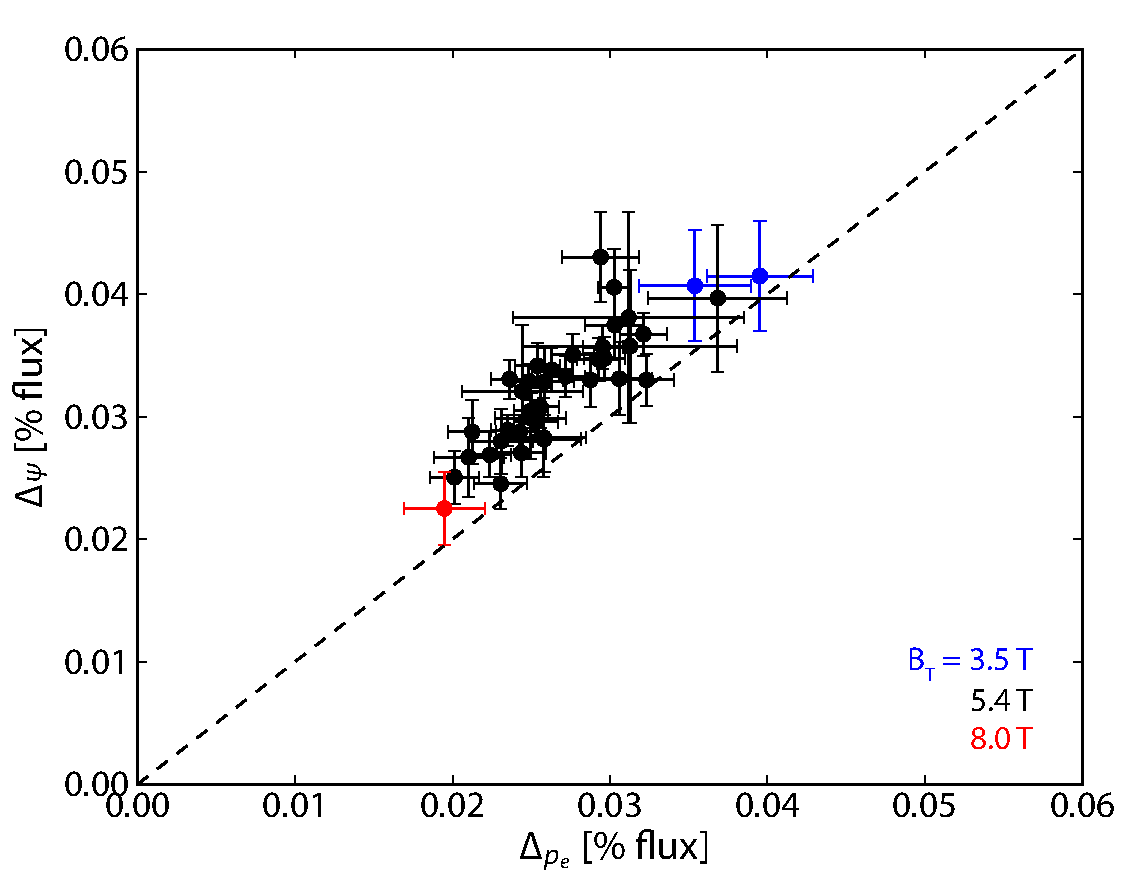
\includegraphics[width=75mm]{graphics/ELMy/deltap_deltapsi.pdf}}{\caption{Comparison of the directly-measured pressure pedestal width and the EPED width $\Delta_\psi$ defined as the average of $\Delta_{n_e}$ and $\Delta_{T_e}$.  The widths trend quite closely to one another, although $\Delta_\psi$ is systematically somewhat wider.}\label{fig:elmy_deltap_deltapsi}}
 \end{floatrow}
\end{figure}

\section{ELM Cycle Synchronization}\label{sec:elmy_sync}

The common practice for modeling the ELMy H-mode pedestal is to take profile data immediately preceding the ELM crash (commonly, data from the last 20\% of the ELM cycle), as this most closely corresponds to the pedestal profile at the stability limit associated with the ELM trigger.  However, as the ELM cycle in H-mode on C-Mod is typically at a comparable repetition rate to the Thomson Scattering system ($\SI{60}{\hertz}$), this practice is only possible on a subset of discharges, with sufficiently long, steady H-mode phases, such that a sufficient number of frames in the desired time wondow can be found.

\begin{figure}[h]
 \pushtooutside
 \fcapside[60mm]{\caption{Comparison of the pressure pedestal height $p_{ped}$ between the ensemble-averaged and ELM-synchronized profiles.  On average, ELM synchronization results in a 10.8\% increase in measured pedestal pressure, consistent with ELM losses observed on other machines.  At lower pressures, ELMs are typically small enough that the perturbation is minimal; however, the distinction becomes important for the highest-pressure ELMy H-modes on C-Mod.}\label{fig:elmy_pped_ens_elmsync}}{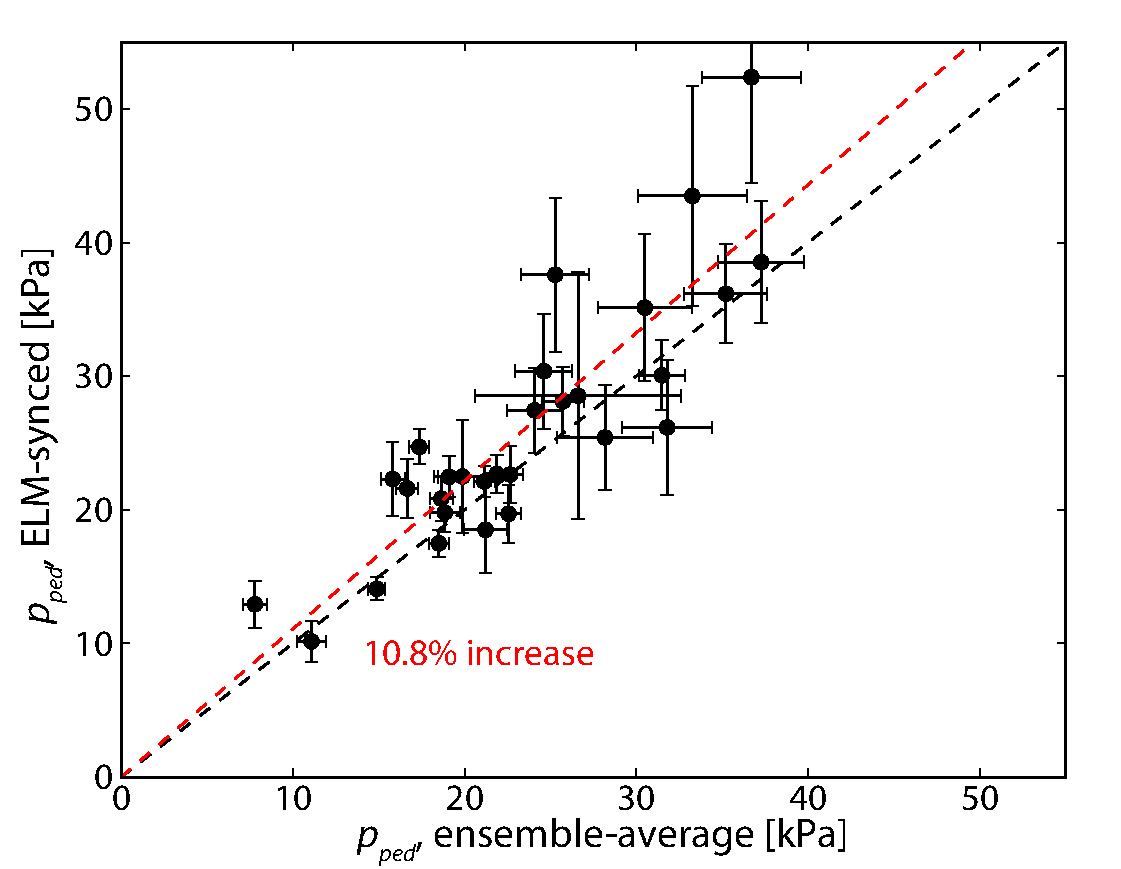
\includegraphics[width=100mm]{graphics/ELMy/pped_ensemble_elmsync.pdf}}
\end{figure}

\begin{figure}[h]
 \pushtooutside
 \fcapside[60mm]{\caption{Comparison of the pressure at the 95\% flux surface, $p_{95}$, between the ensemble-averaged and ELM-synchronized profiles.  On average, ELM synchronization results in a 7.6\% increase in the measured pressure.  This is consistent with the ELM perturbation to the pedestal being largely restricted to the pedestal just within the steep-gradient region, with decreasing perturbation further into the plasma from the pedestal.}\label{fig:elmy_p95_ens_elmsync}}{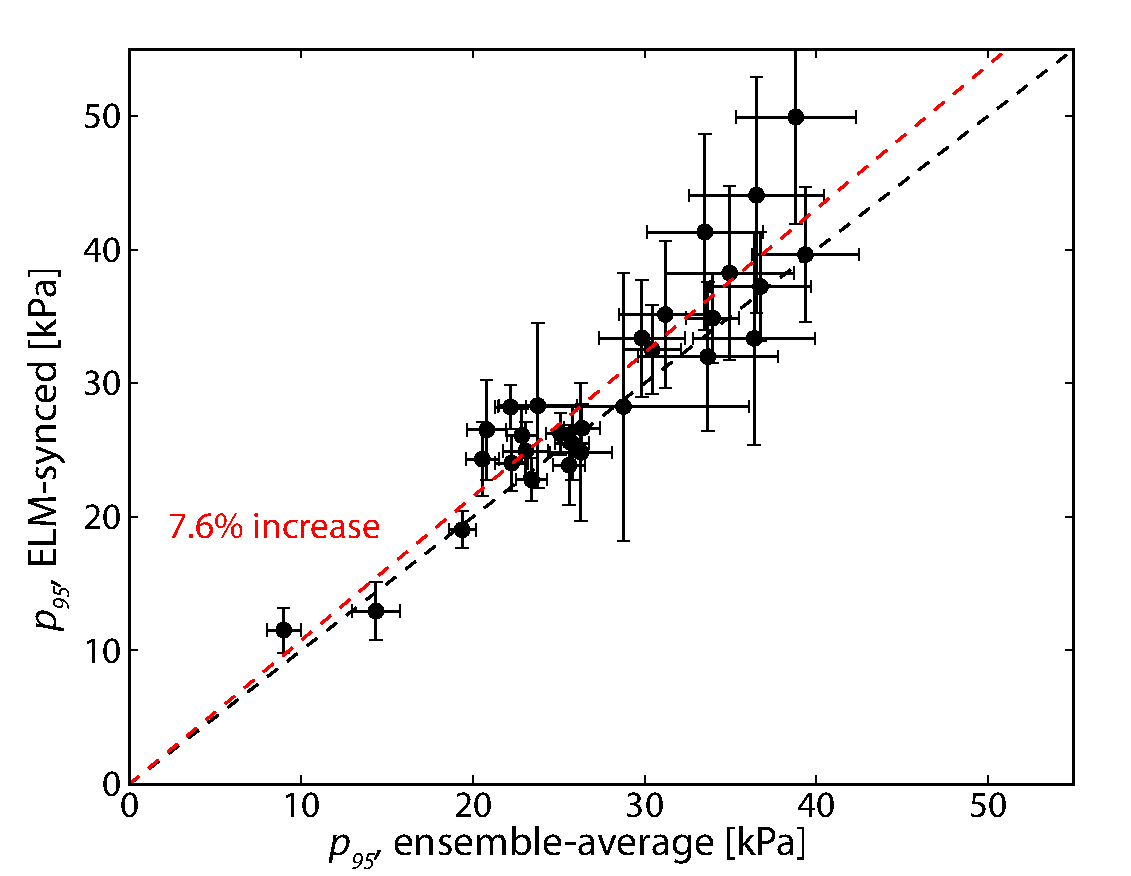
\includegraphics[width=100mm]{graphics/ELMy/p95_ensemble_elmsync.pdf}}
\end{figure}

A comparison between the ensemble-averaged and ELM-synchronized pressure pedestals (pedestal height $p_{ped}$ and the pressure at the 95\% flux surface $p_{95}$) are shown in \cref{fig:elmy_pped_ens_elmsync,fig:elmy_p95_ens_elmsync}.  ELM synchronization finds an average 10.8\% increase in the measured pressure $p_{ped}$, with a slightly lesser increase of 7.6\% in $p_{95}$.  This is consistent with the perturbation to the pressure pedestal by the ELM observed on other machines\gnote{cite?}.  The weaker perturbation due to the ELM crash observed at the 95\% flux surface is also consistent with previous ELM observations -- the ELM crash typically alters the pressure profile only in a region just inside the steep-gradient region, with minimal perturbation to profiles in the plasma interior.\nicesectionending

\section{EPED Model Predictions}\label{sec:elmy_eped}

The EPED model, described in \cref{sec:mod_eped}, combines pedestal limits based on coupled peeling-ballooning MHD instabilities \cite{Snyder2004,Wilson2002,Wilson2006} and kinetic-ballooning mode turbulence \cite{Snyder2001}.  These models set two distinct constraints on the pedestal width and height, with peeling-ballooning MHD predicting $p_{ped} \sim \Delta^{3/4}$ and kinetic-ballooning turbulence predicting $p_{ped} \sim \Delta^2$\gnote{figure?}.  The unique intersection of these two constraints provides a predictive value for the pedestal width and height.  The most recent version of the model, EPED1.63, utilizes gyrokinetic calculations to more accurately constrain the KBM limit, and includes a modified term accounting for the strong diamagnetic stabilization of high-$n$ modes in the pedestal on C-Mod.  A comparison between the observed and predicted pedestal parameters is presented here.

\subsection{Pedestal Height}\label{subsec:elmy_eped_height}

A comparison between the pressure pedestal height predicted by EPED1.63 and the observed height is shown in \cref{fig:elmy_pped_EPED_meas}.  While most measured pedestals lie within the $\pm 20\%$ expected error in the EPED prediction (indicated by the grey band in \cref{fig:elmy_pped_EPED_meas}), the EPED model systematically over-predicts the pedestal pressure, corresponding on average ratio of measured to predicted pedestal heights of $0.84$\gnote{get number!!!}, indicated by the red dashed line.

\begin{figure}[h]
 \pushtooutside
 \fcapside[60mm]{\caption{Pressure pedestal height predicted by EPED1.63 versus the measured (ensemble-averaged) pedestal height, color-coded by magnetic field set.  The grey band indicates perfect agreement, $\pm 20\%$ typical prediction accuracy for EPED.  The EPED model systematically over-predicts the pedestal pressure, with an average match of \note{find number} (indicated by the red line).}\label{fig:elmy_pped_EPED_meas}}{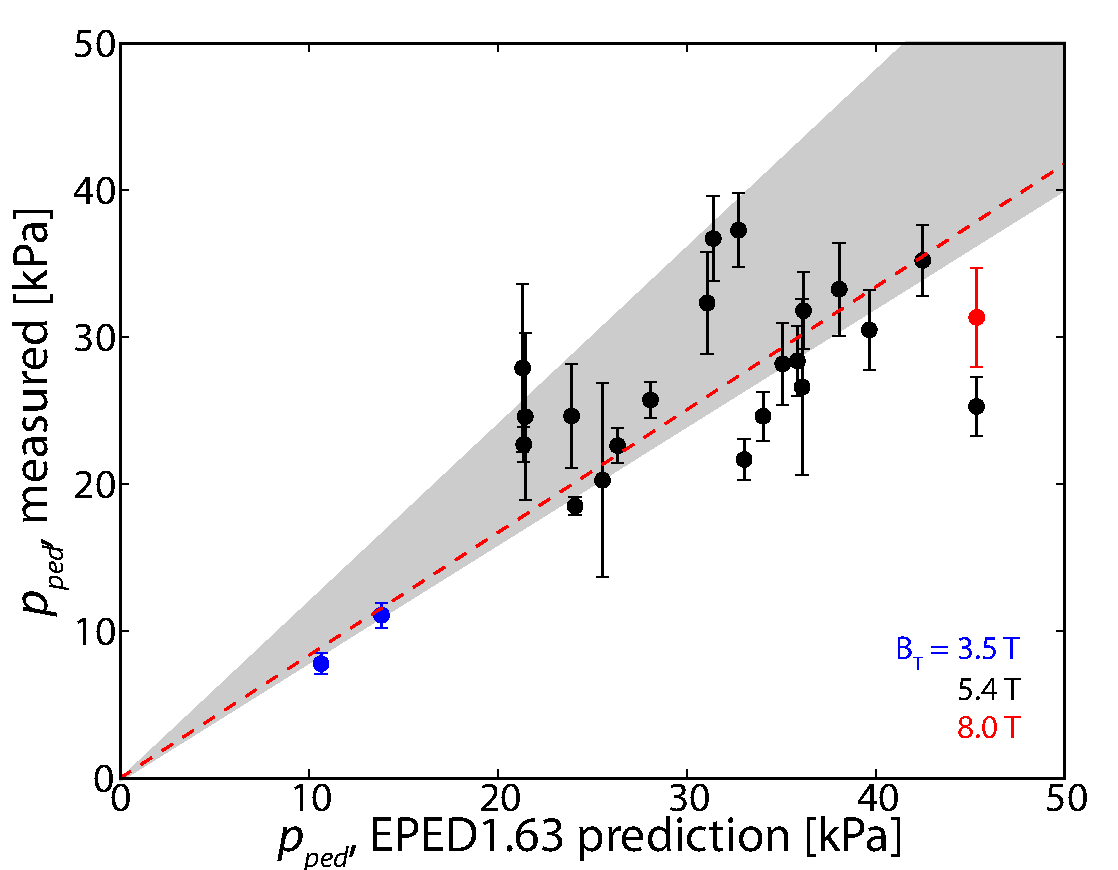
\includegraphics[width=100mm]{graphics/ELMy/pped_EPED_meas.pdf}}
\end{figure}

The discrepancy between the predicted and measured pedestal heights may be attributed (at least in part) to the use of pedestal measurements averaged across the entire ELM cycle (``ensemble-averaged'').  As discussed in \cref{sec:elmy_sync}, models of the pedestal structure (including EPED) most closely correspond to the pedestal structure immediately preceding the ELM crash, where the pedestal is most unstable to the ELM trigger.  A subset of ELMy H-modes are prepared with ELM-synchronized data, shown in \cref{fig:elmy_pped_EPED_sync} with the corresponding ensemble-averaged points for comparison.  The prediction accuracy is substantially improved, with an average ratio of measured to predicted pedestal heights of $0.94$\gnote{get number!!!}, well within the anticipated $\pm 20\%$ accuracy of the EPED prediction.  As expected, the modification to the measured pedestal pressure by ELM synchronization is minimal at lower pedestal pressures, but becomes substantial at higher pedestal pressures ($> \SI{35}{\kilo\pascal}$) as ELM losses increase proportionally with the pedestal stored energy.

The EPED model still systematically slightly over-predicts the pedestal pressure, however -- this is potentially due to the strong sensitivity of the stability calculation to diamagnetic effects, which tend to stabilize higher-$n$ ballooning modes.  As diamagnetic effects are substantial in the relatively collisional pedestal found in H-modes on C-Mod, a careful accounting of these effects is necessary for accurate prediction -- use of a slightly weaker diamagnetic stabilization model brings the prediction into generally better agreement with C-Mod data.

\begin{figure}[t]
 \pushtooutside
 \fcapside[60mm]{\caption{Pressure pedestal height predicted by EPED1.63 versus measured, ELM-synchronized pedestal height (red, with corresponding ensemble-average points shown in black).  The grey band indicates perfect agreement, $\pm 20\%$ typical prediction accuracy for EPED.  ELM synchronization brings the measured pedestal height into better agreement with EPED predictions, with a correspondence of \note{number} (indicated by the red dash).}\label{fig:elmy_pped_EPED_sync}}{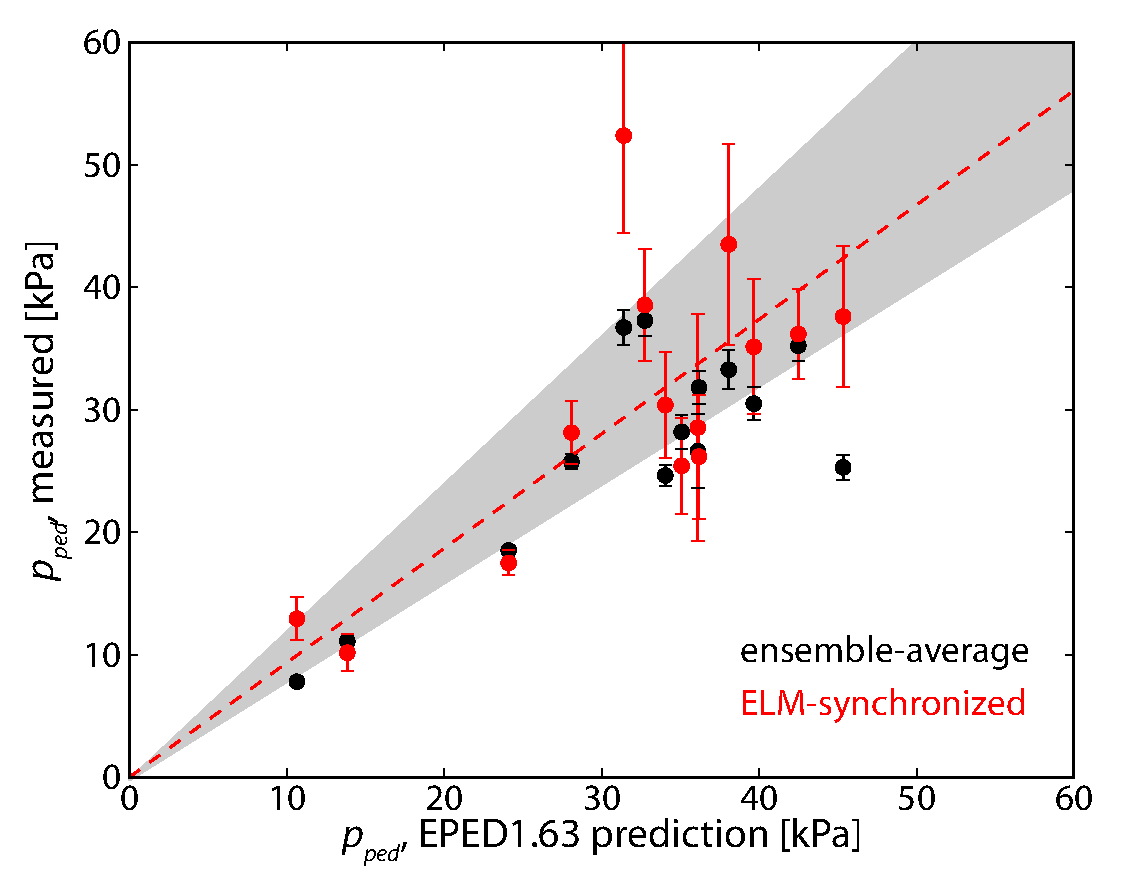
\includegraphics[width=100mm]{graphics/ELMy/pped_EPED_elmsync.pdf}}
\end{figure}

\subsection{Pedestal Width}\label{subsec:elmy_eped_width}

While historically a number of models for the pedestal width (see \cref{sec:mod_empirical}) have been examined, the most uniformly successful has been an expected scaling of pedestal width with poloidal beta at the pedestal top ($\beta_{p,ped}$), observed on several machines \note{cites}, and shown to follow from a critical-gradient limit in the edge pressure profile established by kinetic-ballooning mode (KBM) turbulence \note{cites}.  Including magnetic shear stabilization\gnote{check}, this takes the form $\Delta = c \beta_{p,ped}^{1/2}$, where $c$ is, strictly, a weakly-varying function of a number of plasma parameters.  This constraint on the pedestal width and height is utilized in the EPED model, coupled with peeling-ballooning MHD stability limits to set a unique constraint on the pedestal structure at the ELM crash.

An evaluation of this scaling with ensemble-averaged data is shown in \cref{fig:elmy_betap_deltapsi_all}, with a fitted scale factor of $\langle c \rangle = 0.0857 \pm$\gnote{find errorbar!}, consistent with previously-observed scalings\gnote{cite!}.  The earliest versions of the EPED model used this simple constraint as the second condition on the pedestal width and height, using an experimentally-determined fixed scale factor.  The newest version of the model self-consistently calculates the scale factor from gyrokinetic considerations of the KBM turbulence; however, the results is quantitatively similar.  A comparison of the experimental versus the EPED1.63-predicted pedestals in $\Delta_\psi - \beta_{p,ped}$ space is shown in \cref{fig:elmy_betap_deltapsi_EPED}.

\begin{figure}[ht]
 \pushtooutside
 \fcapside[60mm]{\caption{Ensemble-averaged EPED width $\Delta_\psi$ (\cref{eq:wid_eped}) versus $\beta_{p,ped}$, color-coded by field set.  The expected scaling from the KBM limit, $\Delta_\psi = c \beta_{p,ped}^{1/2}$, is shown with a scale factor of $0.0857$, consistent with observations in previous experiments.}\label{fig:elmy_betap_deltapsi_all}}{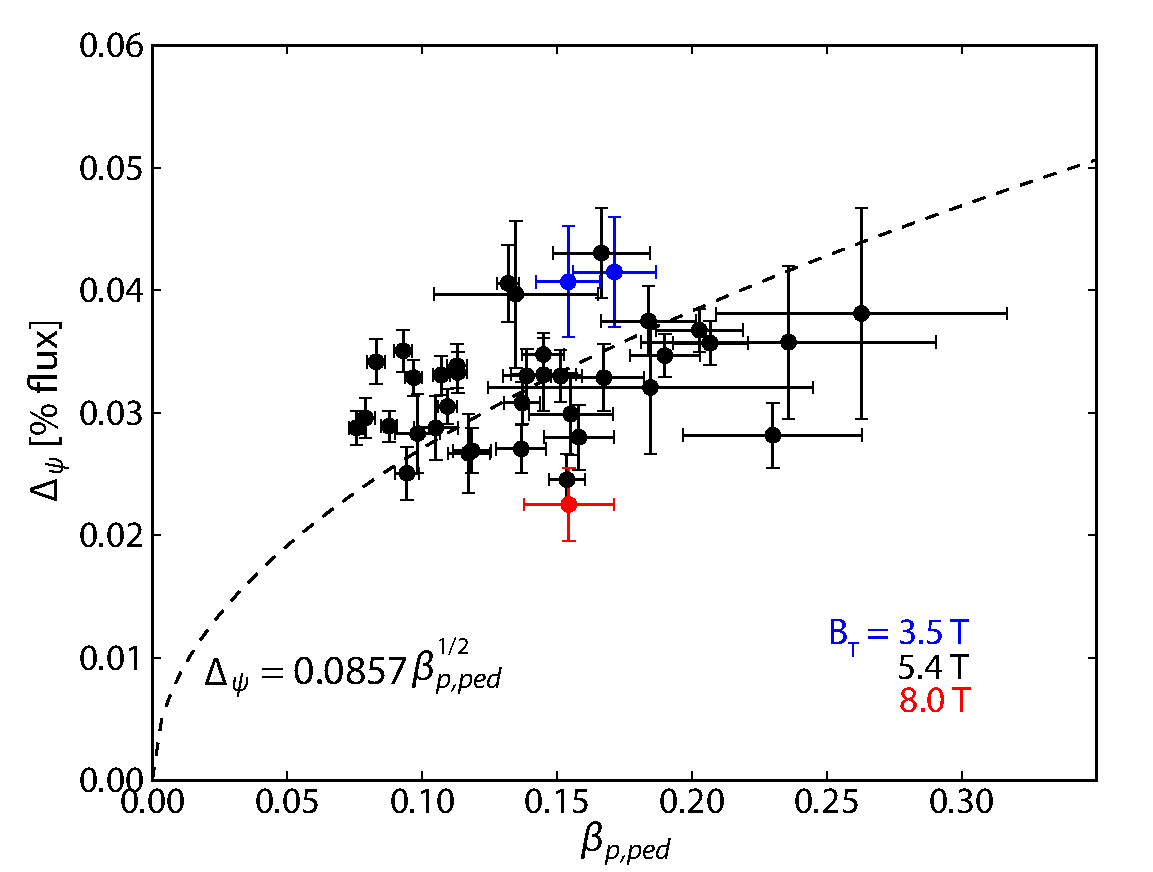
\includegraphics[width=100mm]{graphics/ELMy/betap_deltapsi_all.pdf}}
\end{figure}

\begin{figure}[ht]
 \pushtooutside
 \fcapside[60mm]{\caption{Comparison of EPED1.63-predicted pedestal width $\Delta_\psi$ and height $\beta_{p,ped}$ with the corresponding ensemble-averaged experimental points, with the KBM scaling $\Delta_\psi = c \beta_{p,ped}^{1/2}$.  Though the EPED predictions were calculated with a self-consistent treatment of the scale factor $c$ as a weakly-varying function of plasma parameters, the result is quantitatively similar to the simple fixed scale factor.}\label{fig:elmy_betap_deltapsi_EPED}}{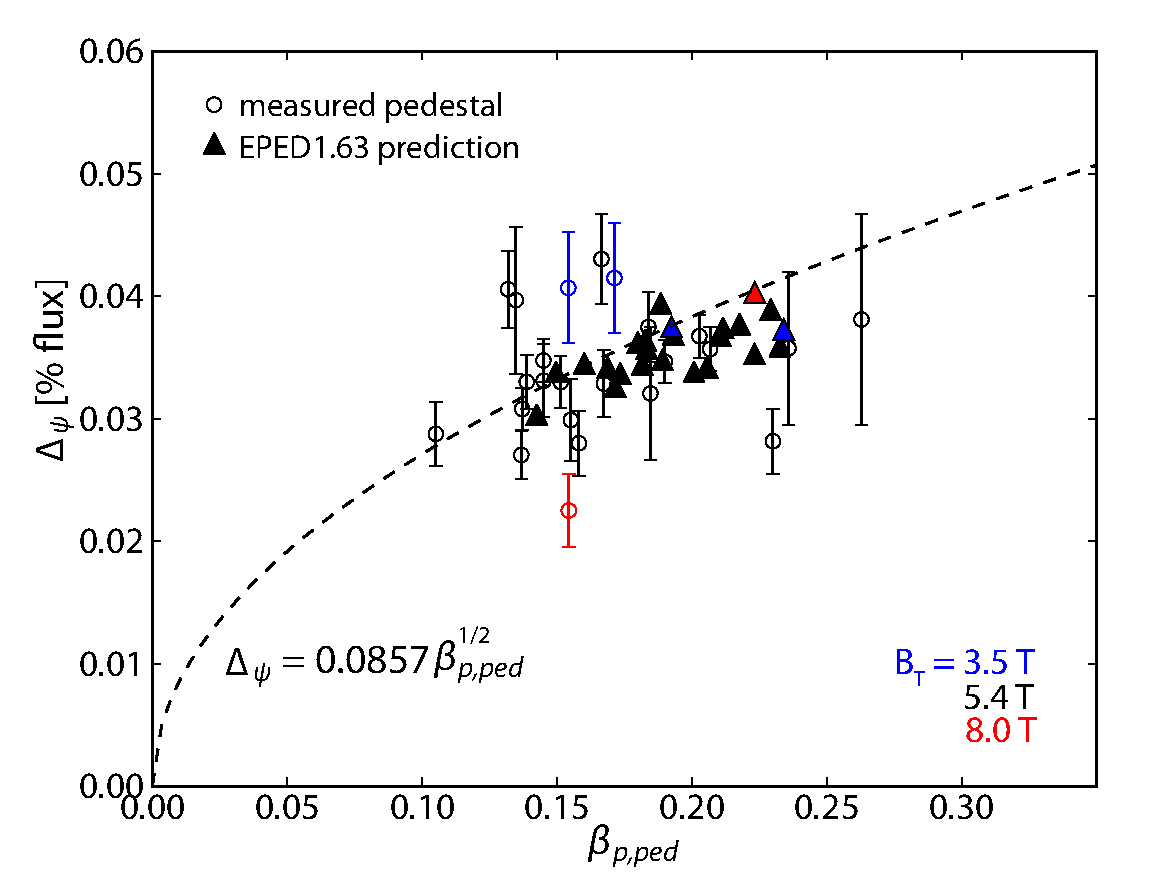
\includegraphics[width=100mm]{graphics/ELMy/betap_deltapsi_EPED.pdf}}
\end{figure}

Application of the ELM synchronization technique does not significantly alter this result, although the pedestal pressure (\ie $\beta_{p,ped}$) is significantly increased in the last 20\% of the ELM cycle.  Recent research in the inter-ELM development of the pedestal \cite{Diallo2014} has shown that the KBM saturates early in the ELM cycle, limiting the pedestal gradient; the pedestal width and height then both increase until the peeling-ballooning MHD boundary is also reached, triggering the ELM.  Consistent with this, ELM-synchronized pedestals exhibit wider, taller pedestals on average, with a similar constraint imposed by the KBM compared to the ensemble-averaged result\gnote{check reasoning!}.  A comparison of the ensemble-averaged and ELM-synced pedestals in $\Delta_\psi - \beta_{p,ped}$ space is shown in \cref{fig:elmy_betap_deltapsi_elmsync}, with the ELM-synced pedestals fitted to a scale factor $\langle c \rangle = 0.0896 \pm $\gnote{get errorbar!}.  The data may be clarified significantly by taking an error-weighted average within fixed bins in $\beta_{p,ped}$ as well, shown in \cref{fig:elmy_betap_deltapsi_betabin}, which tends to reduce the influence of strongly-outlying points on the fit.  Again, the fit is quantitatively very similar -- the data fit well to $\Delta_psi = c \beta_{p,ped}^{1/2}$ with $\langle c \rangle = 0.0851 \pm 0.003$.  Alternately, we may use a more general power-law fit $\Delta_\psi = c_1 \beta_{p,ped}^{c_2}$, with which we find $\langle c_1 \rangle = 0.0824 \pm 0.015$ and $\langle c_2 \rangle = 0.49 \pm 0.11$, closely reproducing the $\beta_{p,ped}^{1/2}$ model.  The fitting results are quite consistent across these methods, demonstrating the robustness of the KBM model for the pedestal width and its insensitivity to the details of data preparation.

\begin{figure}
 \pushtooutside
 \fcapside[60mm]{\caption{Comparison of ensemble-averaged (black) and ELM-synchronized (Red) pedestal width and height, compared to the KBM constraint.  The $\Delta_\psi = 0.0857 \beta_{p,ped}^{1/2}$ scaling found in the ensemble-averaged case is shown in black, while the minor modification of $\Delta_\psi = 0.0896 \beta_{p,ped}^{1/2}$ for the ELM-synced cases is shown in red.}\label{fig:elmy_betap_deltapsi_elmsync}}{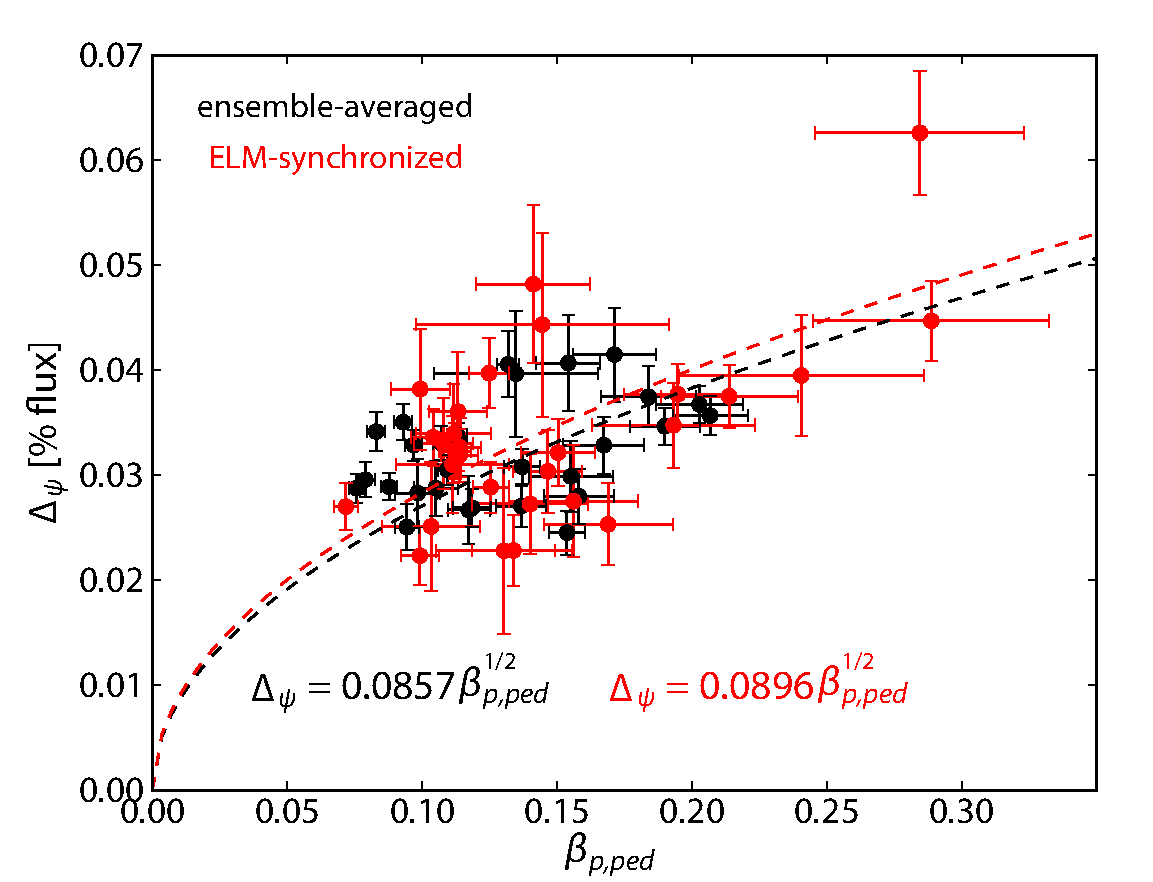
\includegraphics[width=100mm]{graphics/ELMy/betap_deltapsi_elmsync.pdf}}
\end{figure}

\begin{figure}
 \pushtooutside
 \fcapside[60mm]{\caption{ELM-synchronized pedestals, with data binned by $\beta_{p,ped}$ for clarity.  The data are fitted by $\Delta_\psi = (0.0851 \pm 0.003) \beta_{p,ped}^{1/2}$ (black), or by $\Delta_\psi = (0.0824 \pm 0.015) \beta_{p,ped}^{0.49 \pm 0.11}$ using a more general power law.}\label{fig:elmy_betap_deltapsi_betabin}}{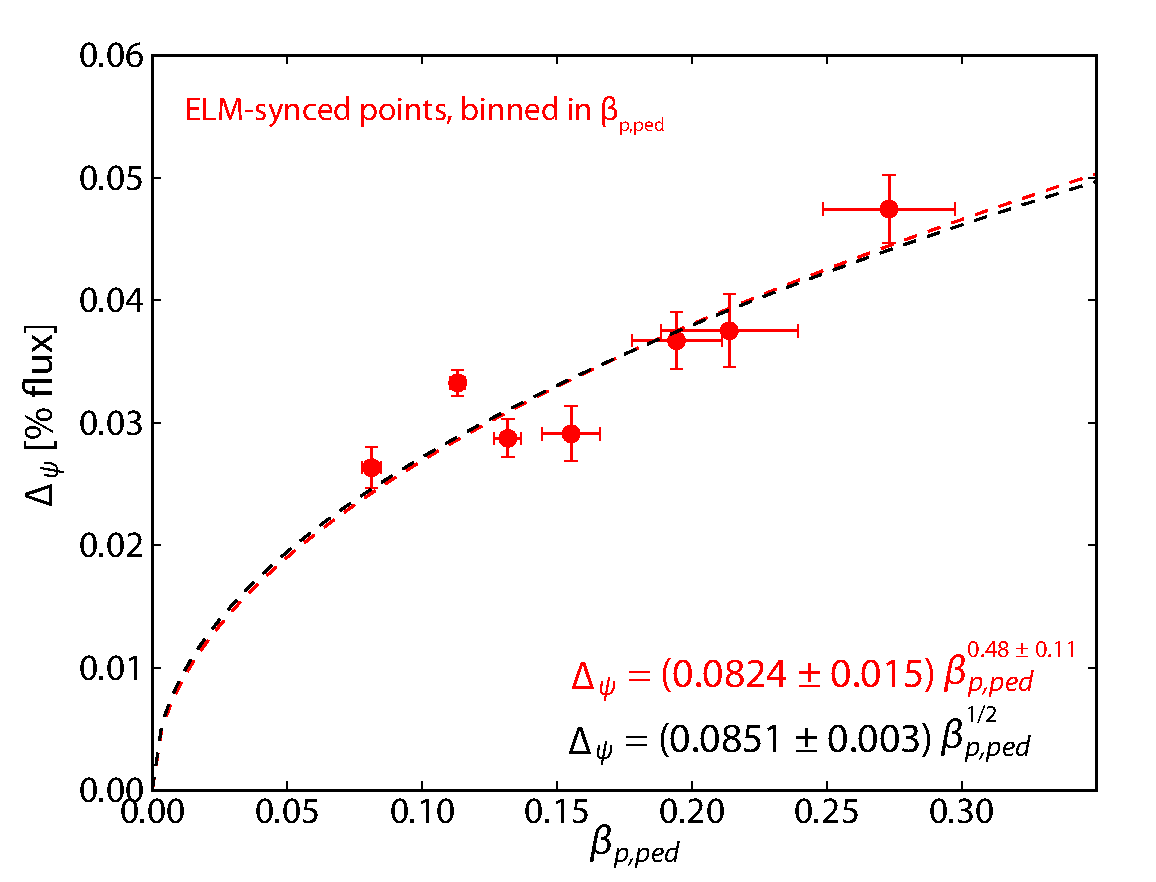
\includegraphics[width=100mm]{graphics/ELMy/betap_deltapsi_elmsync_betabin.pdf}}
\end{figure}

Prediction of the pedestal width is difficult, given the robust width of the pressure pedestal (typically 3-5\% of poloidal flux space, corresponding to $\sim \SI{5}{\milli\meter}$ on C-Mod).  The EPED model correctly recovers this robustness (within the expected $\pm 20\%$ prediction error), as shown in \cref{fig:elmy_deltapsi_eped}.

\begin{figure}
 \pushtooutside
 \fcapside[60mm]{\caption{}\label{fig:elmy_deltapsi_eped}}{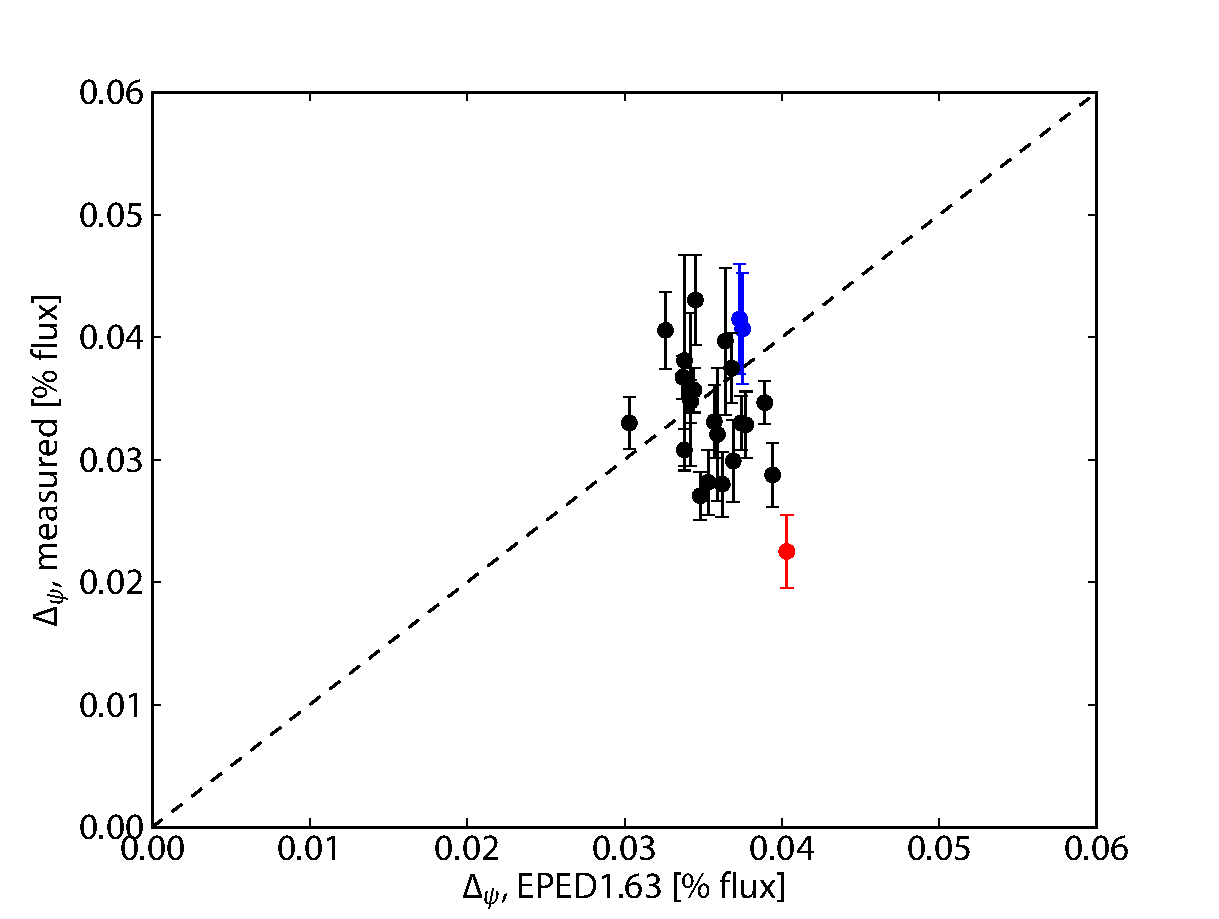
\includegraphics[width=100mm]{graphics/ELMy/deltapsi_EPED_meas.pdf}}
\end{figure}


\nicesectionending

\section{Engineering Parameter Scan}\label{sec:elmy_engineer}

\subsection{$I_p$ Scan}\label{subsec:elmy_ip}

\subsection{Power Scan}\label{subsec:elmy_power}

\nicesectionending

\section{Pedestal Width Response}\label{sec:elmy_width}

\nicechapterending

\bibliographystyle{../plainurl}
\bibliography{../references}